\documentclass{article}

%% Page Margins %%
\usepackage{geometry}
\geometry{
    top = 0.75in,
    bottom = 0.75in,
    right = 0.75in,
    left = 0.75in,
}

\usepackage{amsmath}
\usepackage{graphicx}
\usepackage{parskip}

\title{Assembly Project: Magical Drop}

% TODO: Enter your name
\author{Selim Affes}

\begin{document}
\maketitle

\section{Instruction and Summary}

\begin{enumerate}
\item Which milestones were implemented?
% TODO: List the milestone(s) and in the case of
%       Milestones 4 & 5, list what features you
%       implemented, sorted into easy and hard
%       categories.
\begin{enumerate}
\item Milestones 1, 2 and 3 were all implemented: The playing field is a 7x14 grid. It contains random rows of 4-color bubbles that descend every 100 frames.

\item The character is drawn at the bottom, and can be moved left and right with A and D (it is limited by the board's borders). Under it is the color of the held bubbles, if any.

\item Bubbles can be taken from the board with S, at which point they are held and can be thrown with W. A throw triggers a match if there are enough stacked bubbles (3), which deletes the matched bubbles from the board.

\item The game ends when the rows reach the bottom row, or when the user presses Q to quit.

\item As for further features, I have implemented easy feature 1 through a frame timer (not the clock). What could be considered a part of hard feature 9 is the ``impact frames'', which show matched bubbles before they disappear.
\end{enumerate}
\item How to view the game:
% TODO: specify the pixes/unit, width and height of
%       your game, etc.  NOTE: list these details in
%       the header of your breakout.asm file too!
\begin{enumerate}
\item My game is shown on a 256x256 display with 8px units (32x32 units). The game board is a 7x14-unit grid surrounded by a 9x16-unit grey border.

\item The display's base address is \$gp: 0x10008000; the keyboard MMIO is at 0xffff0000.
\end{enumerate}

\begin{figure}[ht!]
    \centering
    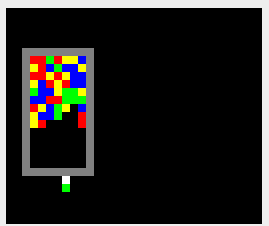
\includegraphics[width=0.7\textwidth]{game_board.png}
    \caption{Example view of the game board}
    \label{game_board}
\end{figure}
\item Game Summary:
% TODO: Tell us a little about your game.
\begin{itemize}
\item This game is a simplified version of Magical Drop written in MIPS Assembly, which I've been making and testing on the MARS simulator. It is played with bubbles hanging from the top of a 7-column, 14-row playfield, moving down over time. The game ends when the bubbles reach the bottom of the board. The player, who stands right under the board, can grab same-colored bubbles and try to make vertical matches of at least 3 bubbles of the same color.

\item Controls:
\begin{itemize}
\item A: Move left

\item D: Move right

\item S: Grab bubbles. You can hold multiple bubbles of the same color. The color of the bubbles you grabbed is shown under the player character.

\item W: Throw the bubbles you grabbed back onto the board

\item Q: Quit
\end{itemize}
\end{itemize}
\item Technical details
\begin{itemize}
\item The board state, containing the color of each cell (black if empty, otherwise the bubble's color), is stored row by row in the 98-word array \texttt{BOARD}, which starts empty. The character's position (its column on the \emph{display}) is stored in the variable \texttt{CHARA}. The variable \texttt{BOX\_OFFSET} stores the byte offset of the first board cell on the display (780), and is used for conversions.

\item Coordinate conversions. Since the game uses both board addresses (the array) and display addresses (the bitmap display), here are the conversions between them:

\begin{table}[h]
\centering
\caption{Conversion table}\vspace{2mm}
\label{conversion_table}
\begin{tabular}{|l|l|l|}
\hline
\textbf{From} & \textbf{To} & \textbf{Formula} \\
\hline
Board cell (row, col) & \texttt{BOARD} address $B$ & $B + 4\,(7 \cdot row + col)$ \\
Board cell (row, col) & Display address ($A$ = \texttt{ADDR\_DSPL}) & $A + 780 + 4\,(32 \cdot row + col)$ \\
Player position \texttt{CHARA} $C$ & Board column & $C - 3$ \\
Player position \texttt{CHARA} $C$ & Display address & $A + 2688 + 4\,C$ \\
\hline
\end{tabular}
\end{table}

Note that $2688 = 21 \cdot 128$ is the start of the character's row on the display.

\item Register roles. Throughout the project, here is how I mainly use registers:

\begin{table}[ht]
\centering
\caption{Register roles}
\begin{tabular}{|c|l|}
\hline
\textbf{Register} & \textbf{Role} \\
\hline
\texttt{\$t0} & Base address of \texttt{BOARD} \\
\texttt{\$t1} & Keyboard MMIO address \\
\texttt{\$t2} & Display base address \\
\texttt{\$t3} & \texttt{BOX\_OFFSET} while drawing, or \texttt{CHARA} while throwing \\
\texttt{\$t4}--\texttt{\$t9} & Loop counters, addresses and colours, local to each routine \\
\texttt{\$s0} & Frame counter for row advancement; kept across the whole game \\
\texttt{\$sp} & Stack, used to save \texttt{\$ra} (and any values needed after a nested call) \\
\hline
\end{tabular}

\end{table}
\end{itemize}


\item Code execution
\begin{enumerate}
\item The setup is done in \texttt{main}. First, we draw the board's grey border, fill the first 4 rows of the board randomly, draw the player in the center, and set the frame counter \$s0 to 0. Then the game loop starts.
\item A standard frame of the game loop goes as follows:
\begin{enumerate}
\item Reload the base addresses \$t0, \$t1 and \$t2 (just in case)

\item Check for keyboard input. If there is any, go to its handler and execute the action

\item Run a game over check

\item Redraw the game field with \texttt{draw\_board}

\item Increment the frame counter; every 100 frames, advance the rows and reset the counter

\item Sleep 16 ms (about 1/60 of a second)

\end{enumerate}

\begin{figure}[ht!]
    \centering
    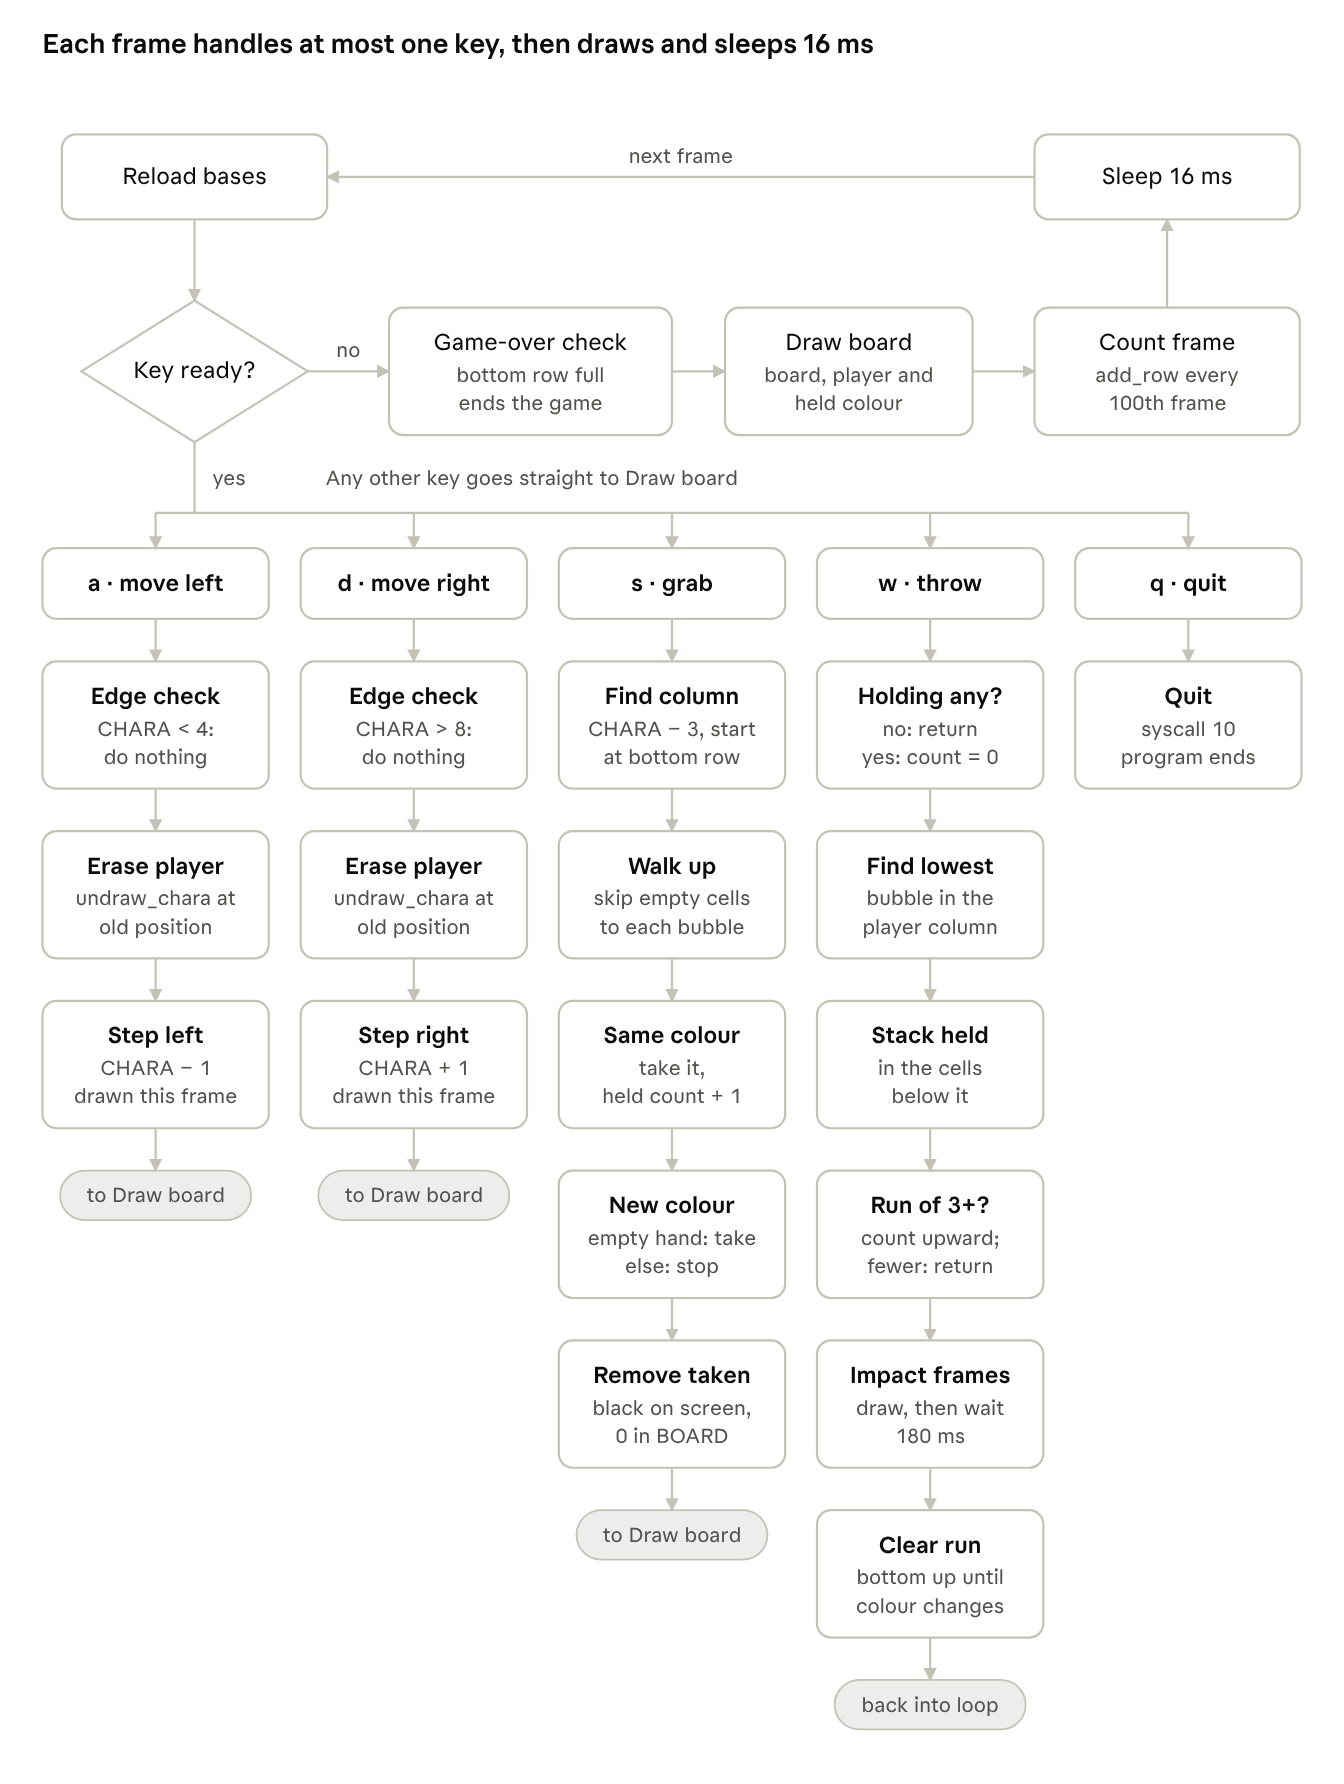
\includegraphics[width=0.7\textwidth]{diagram.png}
    \caption{Detailed diagram of a game loop}
    \label{game_loop}
\end{figure}

\end{enumerate}

\end{enumerate}

\section{Attribution Table}
% TODO: If you worked in partners, tell us who was
%       responsible for which features. Some reweighting
%       might be possible in cases where one group member
%       deserves extra credit for the work they put in.

\begin{center}
\begin{tabular}{|| c ||}
\hline
 Selim Affes, 1011314436, worked alone\\
 \hline
\end{tabular}
\end{center}

% TODO: Fill out the remainder of the document as you see
%       fit, including as much detail as you think
%       necessary to better understand your code.
%       You can add extra sections and subsections to
%       help us understand why you deserve marks for
%       features that were more challenging than they
%       might initially seem.


\end{document}
